\themaG
\graphicspath{{../../S02_Les_angles/Images/}}

\chapter{Les angles}
\label{S02}

%%%%%%%%%%%%%%%%%%%%%%%%%%%%%%%%%%%%%%%%%
%%%%%%%%%%%%%%%%%%%%%%%%%%%%%%%%%%%%%%%%%
\begin{prerequis}
   \begin{itemize}
      \item Caractérisation angulaire du parallélisme : angles alternes-internes, angles correspondants.
   \end{itemize}
\end{prerequis}

\vfill

\begin{debat}[Débat : angles et coordonnées géographiques]
   Tout point à la surface de la Terre est déterminé par ses coordonnées géographiques (la latitude et la longitude) et par son altitude (élévation par rapport au niveau de la mer).
   \begin{itemize}
      \item La {\bf latitude} d'un point sur la Terre est la mesure de l'angle que forment le plan de l'équateur et la demi-droite joignant le centre de la Terre à ce point.
      \item La {\bf longitude} d'un point est l'angle que fait le demi-plan passant par le méridien de ce point avec le plan du méridien de Greenwich.\end{itemize}
   \begin{center}
      \includegraphics[width=5.5cm]{Long_lat}
   \end{center} 
   Le collège Simone Veil se trouve à une latitude de 43,62 degrés Nord et 3,85 degrés Est.
  \bigskip
   \begin{cadre}[B2][F4]
      \begin{center}
         Vidéo : \href{https://www.youtube.com/watch?v=lpYEuHeecko}{{\bf Les fondamentaux : latitude et longitude}, chaîne YouTube {\it La Classe d'Histoire}.}
      \end{center}
   \end{cadre}
\end{debat}

\vfill

\textcolor{PartieGeometrie}{\sffamily\bfseries Cahier de compétences} : chapitre 9, exercices 1 à 9.


%%%%%%%%%%%%%%%%%%%%%%%%%%%%%%%%%%
%%%%%%%%%%%%%%%%%%%%%%%%%%%%%%%%%%
\activites

\begin{activite}[Couples d'angles]
   {\bf Objectif :} faire découvrir la notion d'angles-internes et d'angles correspondants.
   \begin{QCM}
   \partie[préparation]
      Découper les trois bandelettes en bas de page. Ces bandes représentent deux droites $(d_1)$ et $(d_2)$ et une troisième droite $(\Delta)$ qui leur est sécante aux points $A$ et $B$. Placer une attache parisienne au niveau du point $A$ commun entre $(d_1)$ et $(\Delta)$ et une autre au niveau du point $B$ commun entre $(d_2)$ et $(\Delta)$. \\
      Combien d'angles sont-ils matérialisés par cette configuration ? \pf \smallskip
   \partie[angles alternes-internes]
   \ \\ [-11mm]
      \begin{enumerate}
         \item Prendre deux jetons, les placer sur deux angles vérifiant les conditions suivantes :
            \begin{itemize}
               \item les deux angles n'ont pas le même sommet ;
               \item ils sont situés de part et d'autre de la droite $(\Delta)$ ;
               \item ils sont situés \og entre \fg{} les droites $(d_1)$ et $(d_2)$.
            \end{itemize}
         Quelle est la mesure en degrés de chacun de ces deux angles ? \pf
         \item Combien y a-t-il de telles paires d'angles ? \pf \\
         Les angles ainsi construits sont dit {\bf alternes-internes}.
         \item Placer les bandelettes de telle sorte que les droites $(d_1)$ et $(d_2)$ soient parallèles, repérer deux angles alternes-internes par deux jetons puis donner la mesure de chacun de ces deux angles. \pf
         \item En observant les résultats de la classe, quelle conjecture peut-on faire ? \pf \\
         \pf \smallskip
      \end{enumerate}
    \partie[angles correspondants]
    \ \\ [-11mm]
      \begin{enumerate}
         \item Prendre deux jetons, les placer sur deux angles vérifiant les conditions suivantes :
            \begin{itemize}
               \item les deux angles n'ont pas le même sommet ;
               \item ils sont situés du même côté que la droite $(\Delta)$ ;
               \item l'un est situé \og entre \fg{} les droites $(d_1)$ et $(d_2)$, l'autre à l'extérieur.
            \end{itemize}
         Quelle est la mesure en degrés de chacun de ces deux angles ? \pf
         \item Combien y a-t-il de telles paires d'angles ? \pf \\
         Les angles ainsi construits sont dit {\bf correspondants}.
         \item Placer les bandelettes de telle sorte que les droites $(d_1)$ et $(d_2)$ soient parallèles, repérer deux angles alternes-internes par deux jetons puis donner la mesure de chacun de ces deux angles. \pf
         \item En observant les résultats de la classe, quelle conjecture peut-on faire ? \pf \\
         \pf \medskip
      \end{enumerate}
   \end{QCM}
   \begin{pspicture}(0.5,1)(17.5,5)
      \psline(0.75,0.75)(17.25,0.75)
      \rput(1,1.1){$(d_1)$}
      \rput(12,1.25){$A$}
      \psline(0.75,2.25)(17.25,2.25)
      \rput(1,2.6){$(\Delta)$}
      \rput(6,2.75){$B$}
      \rput(12,2.75){$A$}
      \psline(0.75,3.75)(17.25,3.75)
      \rput(1,4.1){$(d_2)$}
      \rput(6,4.25){$B$}
      \psdots(12,0.75)(6,2.25)(12,2.25)(6,3.75)
      \psset{linecolor=gray}
      \psframe(0,0)(18,4.5)
      \psline(0,1.5)(18,1.5)
      \psline(0,3)(18,3)
   \end{pspicture}
\end{activite}

%%%%%%%%%%%%%%%%%%%%%%%%%%%%%%%%%%%%%%%
%%%%%%%%%%%%%%%%%%%%%%%%%%%%%%%%%%%%%%%
\cours 

%%%%%%%%%%%%%%%%%%%%%%%%%%%%%%%%%%%%%%%
\section{Mesure d'angles particuliers : rappels}

\begin{minipage}{10cm}
   \begin{pspicture}(-5,0.25)(5,2.5)
      \rput(0,-0.3){O}
      \rput(3.8,0){angle nul : \udeg{0}}
      \pswedge[fillstyle=solid,fillcolor=B2,linecolor=B2](0,0){1.5}{0}{90}
      \rput(2.5,1.5){\parbox{2.1cm}{\textcolor{B2}{angle aigu : \\ \udeg{0} < \pswedge[fillstyle=solid,fillcolor=B2,linecolor=B2](0.2,0){0.3}{0}{90} \qquad < \udeg{90}}}}
      \pswedge[fillstyle=solid,fillcolor=A1,linecolor=A1](0,0){1.5}{90}{180}
      \rput(-2.5,1.5){\parbox{2.5cm}{\textcolor{A1}{angle obtus : \\ \udeg{90} < \pswedge[fillstyle=solid,fillcolor=A1,linecolor=A1](0.4,0){0.3}{90}{180} \quad\; < \udeg{180}}}}
      \rput(0,2.5){angle droit : \udeg{90}}
      \rput(-3.8,0){angle plat : \udeg{180}}
      \psline(-2.5,0)(2.5,0)
      \psline(0,2)
   \end{pspicture}   
\end{minipage}
\begin{minipage}{5.5cm}
   Dans cette configuration, la somme des deux angles mesure \udeg{180}, on dit que ces angles sont supplémentaires. \\
   \begin{pspicture}(7,1.5)
      \psline(0.5,0)(5.5,0)
      \psline(3,0)(1.8,1.2)
      \psarc[linecolor=B1](3,0){0.7}{135}{180}
      \rput(2,0.4){\textcolor{B1}{\udeg{45}}}
      \psarc[linecolor=A1](3,0){0.5}{0}{135}
      \rput(3.6,0.7){\textcolor{A1}{\udeg{135}}}
   \end{pspicture}
\end{minipage}


%%%%%%%%%%%%%%%%%%%%%%%%%%%%%%%%%%%%
\section{Angles alternes-internes et correspondants}

\parbox{8cm}{Lorsque deux droites sont coupées par une droite sécante $(\Delta)$, on obtient huit angles. \\
{\it Dans la suite du cours, on se place dans cette configuration.}}
\hfill
\parbox{6.5cm}{\psset{unit=0.7}
   \begin{pspicture}(-0.5,-0.25)(6,3.5)
      \psline(0,1.5)(6,0.5)
      \psline(1,3)(6,3)
      \psline(1,0)(5,4)
      \psarc[linecolor=B2,doubleline=true](4,3){0.7}{0}{45}
      \rput(5,3.4){\textcolor{B2}{\small $A_2$}}
      \psarc[linecolor=J1,doubleline=true](4,3){0.7}{180}{225}
      \rput(3,2.5){\textcolor{J1}{\small $A_4$}}
      \psarc[linecolor=A1](4,3){0.5}{45}{180}
      \rput(3.7,3.8){\textcolor{A1}{\small $A_1$}}
      \psarc[linecolor=G1](4,3){0.5}{225}{0}
      \rput(4.35,2.25){\textcolor{G1}{\small $A_3$}}
      \psarc[linecolor=B2,doubleline=true](2.15,1.15){0.7}{-10}{45}
      \rput(3.2,1.4){\textcolor{B2}{\small $B_2$}}
      \psarc[linecolor=J1,doubleline=true](2.15,1.15){0.7}{170}{225}
      \rput(1.1,0.7){\textcolor{J1}{\small $B_4$}}
      \psarc[linecolor=A1](2.15,1.15){0.5}{45}{170}
      \rput(1.8,1.9){\textcolor{A1}{\small $B_1$}}
      \psarc[linecolor=G1](2.15,1.15){0.5}{225}{-10}
      \rput(2.4,0.3){\textcolor{G1}{\small $B_3$}}
      \rput(0.7,-0.3){$(\Delta)$}
      \rput(-0.5,1.5){$(d_1)$}
      \rput(0.5,3){$(d_2)$}
   \end{pspicture}}

\begin{definition}
   Deux angles sont {\bf alternes-internes} s'ils n'ont pas le même sommet, qu'ils sont situés de part et d'autre de la sécante $(\Delta)$ et qu'ils se situent \og entre \fg{} les droites $(d_1)$ et $(d_2)$.
\end{definition}

\begin{exemple*1}
Sur la figure, il y a deux couples d'angles alternes-internes : $A_4$ et $B_2$ ; $A_3$ et $B_1$.
\end{exemple*1}

\bigskip

\begin{definition}
   Deux angles sont {\bf correspondants} s'ils n'ont pas le même sommet, qu'ils sont situés du même côté de la sécante $(\Delta)$, l'un entre les deux droites $(d_1)$ et $(d_2)$ et l'autre à l'extérieur.
\end{definition}

\begin{exemple*1}
Sur la figure, il existe quatre couples d'angles correspondants :  $A_1$ et $B_1$ ; $A_2$ et $B_2$ ; $A_3$ et $B_3$ ; $A_4$ et $B_4$.
\end{exemple*1}


%%%%%%%%%%%%%%%%%%%%%%%%%%%%%%%%%%%
\section{Et si les droites sont parallèles ?}

\begin{propriete}
   \begin{itemize}
      \item Si les deux droites $(d_1)$ et $(d_2)$ sont parallèles, alors les angles alternes-internes et les angles correspondants sont égaux deux à deux.
      \item Si deux angles alternes-internes ou deux angles correspondants sont égaux, alors les droites $(d_1)$ et $(d_2)$ sont parallèles.
   \end{itemize}
   \ \\ [-14mm]
\end{propriete}

\begin{exemple}
   {\psset{unit=0.9}
   \begin{pspicture}(0,0.3)(6,3.2)
      \psline(1,1)(6,1)
      \psline(1,2.5)(6,2.5)
      \psline(2,0)(4,3)
      \rput(2.4,2.1){$\alpha =\udeg{56}$}
      \rput(3.5,1.5){$\beta$}
      \rput(1.8,0.5){$\gamma$}
      \psarc[linecolor=B2,doubleline=true](3.67,2.5){0.6}{182}{234}
      \psarc[linecolor=A1,doubleline=true](2.67,1){0.6}{2}{55}
      \psarc[linecolor=J1,doubleline=true](2.67,1){0.6}{182}{233}
      \rput(5.5,1.75){\parbox{1.5cm}{\small droites\\parallèles}}
   \end{pspicture}}
   \correction
   Mesures de $\beta$ et $\gamma$, sachant que les droites sont parallèles :
   \begin{itemize}
      \item $\alpha$ et $\beta$ sont des angles alternes-internes, ils ont donc même mesure. D'où : $\beta =\alpha =\udeg{56}$.
      \item $\alpha$ et $\gamma$ sont des angles correspondants, ils ont donc même mesure. D'où : $\gamma =\alpha =\udeg{56}$.
   \end{itemize}
\end{exemple}


%%%%%%%%%%%%%%%%%%%%%%%%%%%%%%%%%%%%%%
%%%%%%%%%%%%%%%%%%%%%%%%%%%%%%%%%%%%%%
\exercicesbase

\begin{colonne*exercice}

\serie{Angles particuliers} %%%%%%%%%

\begin{exercice} %1
   Au regard de la figure ci-dessous, que peut-on dire des angles :
   \begin{colenumerate}{3}
      \item 1 et 5 ?
      \item 2 et 6 ?
      \item 4 et 6 ?
      \item 3 et 7 ?
      \item 3 et 5 ?
      \item 4 et 8 ?
   \end{colenumerate}
   \begin{pspicture}(-0.5,-0.3)(6,4.5)
      \psline(0,1.5)(6,0.5)
      \psline(1,3)(6,3)
      \psline(1,0)(5,4)
      \psarc(4,3){0.7}{0}{45}
      \rput(5,3.4){2}
      \psarc(4,3){0.7}{180}{225}
      \rput(3,2.5){4}
      \psarc(4,3){0.5}{45}{180}
      \rput(3.7,3.8){1}
      \psarc(4,3){0.5}{225}{0}
      \rput(4.35,2.25){3}
      \psarc(2.15,1.15){0.7}{-10}{45}
      \rput(3.2,1.4){6}
      \psarc(2.15,1.15){0.7}{170}{225}
      \rput(1.1,0.7){8}
      \psarc(2.15,1.15){0.5}{45}{170}
      \rput(1.8,1.9){5}
      \psarc(2.15,1.15){0.5}{225}{-10}
      \rput(2.4,0.3){7}
   \end{pspicture}
\end{exercice}

\begin{corrige}
   \ \\ [-5mm]
   \begin{enumerate}
      \item Les angles 1 et 5 sont {\blue correspondants}.
      \item Les angles 2 et 6 sont {\blue correspondants}.
      \item Les angles 4 et 6 sont {\blue alternes-internes}.
      \item Les angles 3 et 7 sont {\blue correspondants}.
      \item Les angles 3 et 5 sont {\blue alternes-internes}.
      \item Les angles 4 et 8 sont {\blue correspondants}.
   \end{enumerate}
\end{corrige}

\smallskip

\begin{exercice}
   Dans la configuration suivante, citer :
   \begin{enumerate}
       \item la sécante ;
       \item deux angles correspondants ;
       \item deux angles alternes-internes.
   \end{enumerate}
   \begin{pspicture}(-3,-1.7)(3,1.3)
      \psline(-1.5,0)(2,0)
      \psline(-1,0.75)(2,-1.5)
      \psline(-1.5,-1)(2.5,-1)
      \rput(-1.75,0){$x$}
      \rput(-1.2,0.9){$y$}
      \rput(2.25,0){$t$}
      \rput(2.25,-1.6){$s$}
      \rput(2.75,-1){$u$}
      \rput(0.2,0.25){$O$}
      \rput(1.5,-0.75){$I$}
      \rput(-1.75,-1){$k$}
   \end{pspicture}
\end{exercice}

\begin{corrige}
   \ \\ [-5mm]
   \begin{enumerate}
       \item La sécante est {\blue la droite $(ys)$}.
       \item Il y a quatre couples d'angles correspondants : {\blue $\widehat{yOt}$ et $\widehat{OIu}$ ; \, $\widehat{yOx}$ et $\widehat{OIk}$ ; \, $\widehat{tOI}$ et $\widehat{uIs}$ ; \, $\widehat{xOI}$ et $\widehat{kIs}$}.
       \item Il y a deux couples d'angles alternes-internes : {\blue $\widehat{xOI}$ et $\widehat{OIu}$ \quad ; \quad $\widehat{tOI}$ et $\widehat{OIk}$}.
   \end{enumerate}
\end{corrige}

\smallskip

\begin{exercice}
   Sur cette figure, les droites $(xy)$ et $(zt)$, ainsi que les droites $(su)$ et $(fg)$, sont parallèles. \\
   Compléter le tableau suivant lorsque c'est possible.
   \begin{center}
   \psset{xunit=2cm}
      \begin{pspicture}(-1.5,-2.2)(2.5,1.2)
         \psline(-1,0)(2,0)
         \psline(-1,-1)(2,-1)
         \psline(-1,1)(1,-2)
         \psline(0,1)(2,-2)
         \psline(0,-2)(1,1)
         \rput(-1.1,0){$x$}
         \rput(2.1,0){$y$}
         \rput(-1.1,-1){$z$}
         \rput(2.1,-1){$t$}
         \rput(-1.1,1.1){$s$}
         \rput(1.1,-2.1){$u$}
         \rput(-0.1,1.1){$f$}
         \rput(2.1,-2.1){$g$}      
         \rput(-0.1,-2.1){$h$}
         \rput(1.1,1.1){$i$}
         \rput(-0.3,0.25){$A$}
         \rput(0.85,0.2){$B$}
         \rput(0.3,-0.65){$C$}
         \rput(1.4,-0.65){$D$}
      \end{pspicture}
   \end{center}
   \begin{tabular}{|C{2.2}|*{4}{C{0.95}|}}
      \hline
      Angle & $\widehat{yBg}$ & $\widehat{zCi}$ & $\widehat{fBi}$ & $\widehat{uCi}$ \\
      \hline
       Angle alterne-interne & & & & \\
       \hline
       Angle correspondant & & & & \\
       \hline
   \end{tabular}
\end{exercice}

\begin{corrige}
   On obtient le tableau suivant, par exemple : \\ \smallskip
   \begin{tabular}{|C{1.8}|*{4}{C{0.9}|}}
      \hline
      Angle & $\widehat{yBg}$ & $\widehat{zCi}$ & $\widehat{fBi}$ & $\widehat{uCi}$ \\
      \hline
       \footnotesize Angle alterne-interne & \textcolor{blue}{$\widehat{zDf}$} & \textcolor{blue}{$\widehat{hBy}$} & \textcolor{blue}{$\varnothing$} & \textcolor{blue}{$\widehat{fBh}$} \\
       \hline
       \footnotesize Angle correspondant & \textcolor{blue}{$\widehat{tDg}$} \textcolor{blue}{$\widehat{yAu}$} & \textcolor{blue}{$\widehat{xBi}$} & \textcolor{blue}{$\widehat{sCi}$} & \textcolor{blue}{$\widehat{gBi}$} \\
       \hline
   \end{tabular}
\end{corrige}

\medskip

\serie{Droites parallèles} %%%%%%%%%


\begin{exercice}
   Yossra pense que l'une des deux paires de droites $(d_1)$ et $(d_2)$ est parallèle. A-t-elle raison ? \\
   \begin{pspicture}(0,0)(4,3)
      \pstGeonode[PointSymbol=none,PointName=none](0,2.5){A}(4,0){B}(0,1){C}(3,2){D}(1,0){E}(4,1){F}
      \pstInterLL[PointName=none,PointSymbol=none]{A}{B}{C}{D}{H}
       \pstInterLL[PointName=none,PointSymbol=none]{A}{B}{E}{F}{I}
      \pstLineAB{A}{B}
      \pstLineAB{C}{D}
      \pstLineAB{E}{F}
      \pstMarkAngle{D}{H}{A}{\udeg{119}}
      \pstMarkAngle{B}{I}{F}{\udeg{61}}
      \rput(0.5,0.8){$(d_1)$}
      \rput(1.7,-0.2){$(d_2)$}
   \end{pspicture}   
   \begin{pspicture}(-1,0.25)(3.5,3.25)
      \pstGeonode[PointSymbol=none,PointName=none](0,1.5){A}(3,1){B}(0,0){C}(1.5,3){D}(1.5,0){E}(2.5,2.5){F}
      \pstInterLL[PointName=none,PointSymbol=none]{A}{B}{C}{D}{H}
       \pstInterLL[PointName=none,PointSymbol=none]{A}{B}{E}{F}{I}
      \pstLineAB{A}{B}
      \pstLineAB{C}{D}
      \pstLineAB{E}{F}
      \pstMarkAngle{B}{H}{D}{\udeg{59}}
      \pstMarkAngle{E}{I}{B}{\udeg{111}}
      \rput(1,2.8){$(d_1)$}
      \rput(3,2.5){$(d_2)$}
   \end{pspicture}
\end{exercice}

\begin{corrige}
   Oui, Yossra a raison : \\
   \begin{itemize}
      \item Première figure : l'angle supplémentaire à \udeg{119} de l'autre côté de $(d_1)$ vaut $\udeg{180}-\udeg{119} =\udeg{61}$. \\
      On a deux angles correspondants de même mesure donc, {\blue les droites $(d_1)$ et $(d_2)$ sont parallèles}.
      \item Deuxième figure : l'angle supplémentaire à \udeg{111} de l'autre côté de $(d_2)$ vaut $\udeg{180}-\udeg{111} =\udeg{69}$. \\
      On a deux angles alternes-internes de mesures différentes donc, {\blue $(d_1)$ et $(d_2)$ ne sont pas parallèles}.
   \end{itemize}
\end{corrige}

\smallskip

\begin{exercice} %3
   Sur la figure ci-dessous :
   \begin{itemize}
      \item les droites $(ab), (cd)$ et $(ef)$ sont parallèles ;
      \item $R$ est un point de $(ab)$, $S$ un point de $(cd)$ et $T$ un point de $(ef)$ tels que $\widehat{bRS} =\udeg{20}$ et $\widehat{RST} =\udeg{57}$.
   \end{itemize}
   Calculer la mesure de l'angle $\widehat{STf}$. \\
   \begin{pspicture}(-1,0)(7,3.8)
      \pstGeonode[PointSymbol=none,PosAngle={90}](0,0.5){e}(2,0.5){T}(7,0.5){f}(0,2){c}(4,2){S}(7,2){d}(0,3){a}(2,3){R}(7,3){b}
      \pstLineAB{a}{b}
      \pstLineAB{c}{d}
      \pstLineAB{e}{f}
      \pstLineAB{R}{S}
      \pstLineAB{S}{T}
      \pstMarkAngle{S}{R}{b}{}
      \rput(3,2.8){\udeg{20}}
      \pstMarkAngle[MarkAngleType=double]{R}{S}{T}{}
      \rput(3.2,1.8){\udeg{57}}
      \pstMarkAngle{f}{T}{S}{?}
   \end{pspicture}
\end{exercice}

\begin{corrige}
   \begin{itemize}
      \item Les angles $\widehat{bRS}$ et $\widehat{RSc}$ sont alternes-internes et les droites $(ab)$ et $(cd)$ sont parallèles donc : $\widehat{RSc} =\widehat{bRS} =\udeg{20}$.
      \item On décompose l'angle $\widehat{RST}$ : $\widehat{RST} =\widehat{RSc}+\widehat{cST}$ donc, $\widehat{cST} =\widehat{RST} -\widehat{RSc} =\udeg{57}-\udeg{20} =\udeg{37}$.
      \item Les angles $\widehat{cST}$ et $\widehat{STf}$ sont alternes-internes et les droites $(cd)$ et $(ef)$ sont parallèles donc : $\widehat{STf} =\widehat{cST} =\blue \udeg{37}$.
   \end{itemize}
\end{corrige}

\smallskip

\begin{exercice}
   Inès possède un champ en forme de quadrilatère $INES$ dont les côtés $(IN)$ et $(SE)$ sont parallèles. Elle prend la mesure de deux angles et se demande si son quadrilatère peut être un parallélogramme.
   \begin{enumerate}
      \item Écrire sur le schéma ci-dessous la mesure de tous les angles existants.
      \item Les droites $(IS)$ et $(NE)$ sont-elles parallèles ?
      \item Quelle est alors la nature du quadrilatère $INES$ ?
   \end{enumerate}
   \psset{unit=0.7}
   \begin{pspicture}(-1,0)(10,6)
      \pstGeonode[PointSymbol=none,PointName=none](0,1){a}(10,1){b}(0,4){c}(10,4){d}(0.33,0){f}(4,5.5){g}(6.33,0){h}(9,5){j}
      \pstLineAB{a}{b}
      \pstLineAB{c}{d}
      \pstLineAB{f}{g}
      \pstLineAB{h}{j}
      \pstInterLL[PosAngle=-45,PointSymbol=none]{a}{b}{f}{g}{S}
      \pstInterLL[PosAngle=-45,PointSymbol=none]{a}{b}{h}{j}{E}
      \pstInterLL[PosAngle=-45,PointSymbol=none]{c}{d}{f}{g}{I}
      \pstInterLL[PosAngle=-45,PointSymbol=none]{c}{d}{h}{j}{N}
      \pstMarkAngle{j}{N}{I}{\udeg{121}}
      \pstMarkAngle{E}{S}{I}{\udeg{49}}
   \end{pspicture}
\end{exercice}

\begin{corrige}
\ \\ [-5mm]
   \begin{enumerate}
      \item Schéma du terrain d'Inès : \\
      {\psset{unit=0.7}
   \begin{pspicture}(0,-0.5)(10,6)
      \pstGeonode[PointSymbol=none,PointName=none](0,1){a}(10,1){b}(0,4){c}(10,4){d}(0.33,0){f}(4.5,5.5){g}(6.33,0){h}(9,5){j}
      \pstLineAB{a}{b}
      \pstLineAB{c}{d}
      \pstLineAB{f}{g}
      \pstLineAB{h}{j}
      \pstInterLL[PosAngle=-45,PointSymbol=none,PointName=none]{a}{b}{f}{g}{S}
      \pstInterLL[PosAngle=-45,PointSymbol=none,PointName=none]{a}{b}{h}{j}{E}
      \pstInterLL[PosAngle=-45,PointSymbol=none,PointName=none]{c}{d}{f}{g}{I}
      \pstInterLL[PosAngle=-45,PointSymbol=none,PointName=none]{c}{d}{h}{j}{N}
      \pstMarkAngle{j}{N}{I}{\udeg{121}}
      \pstMarkAngle{E}{S}{I}{\udeg{49}}
      \pstMarkAngle{I}{N}{E}{\blue\udeg{59}}
      \pstMarkAngle{E}{N}{d}{\blue\udeg{121}}
      \pstMarkAngle{d}{N}{j}{\blue\udeg{59}}
      \pstMarkAngle{b}{E}{N}{\blue\udeg{59}}
      \pstMarkAngle{h}{E}{b}{\blue\udeg{121}}
      \pstMarkAngle{N}{E}{S}{\blue\udeg{121}}
      \pstMarkAngle{S}{E}{h}{\blue\udeg{59}}
      \pstMarkAngle{f}{S}{E}{\blue\udeg{131}}
      \pstMarkAngle{I}{S}{a}{\blue\udeg{131}}
      \pstMarkAngle{a}{S}{f}{\blue\udeg{49}}
      \pstMarkAngle{f}{S}{E}{\blue\udeg{131}}
      \pstMarkAngle{I}{S}{a}{\blue\udeg{131}}
      \pstMarkAngle{g}{I}{e}{\blue\udeg{49}}
      \pstMarkAngle{e}{I}{f}{\blue\udeg{131}}
      \pstMarkAngle{d}{I}{g}{\blue\udeg{49}}
      \pstMarkAngle{f}{I}{d}{\blue\udeg{131}}
   \end{pspicture}}
      \item Si les droites $(IS)$ ET $(NE)$ étaient parallèles, les angles correspondants en $I$ et $N$ par exemple seraient égaux, ce qui n'est pas le cas ici (\udeg{131}$\neq$\udeg{121}) donc, {\blue ces droites ne sont pas parallèles}.
      \item Dans le quadrilatère $INES$, les droites $(IN)$ et $(SE)$ sont parallèles, mais les droites $(IS)$ et $(EN)$ ne le sont pas donc, {\blue le quadrilatère $INES$ est un trapèze}.   
   \end{enumerate}

\bigskip

\corec{Eratosthène et la circonférence de la Terre} %%%%%

\medskip

$\bullet$ On peut commencer par calculer la distance entre Syène et Alexandrie : \\
un chameau met 50 jours pour faire cette distance et il parcourt 100 stades chaque jour, soit au total $50\times100 \text{ stades} =5\,000$ stades. \\
Sachant qu'un stade mesure 157,5 m, la distance entre ces villes vaut $5\,000\times\um{157,5} =\um{787500}$. \\ \smallskip
$\bullet$ Puis on calcule l'angle $\alpha$ au centre de la Terre : \\
les angles $\alpha$ et \udeg{7,2} sont alternes-internes et on sait que les droites portées par les rayons solaires sont parallèles donc, $\alpha =\udeg{7,2}$. \\ \smallskip
$\bullet$ Ensuite, on calcule la circonférence de la Terre par proportionnalité : \\
\udeg{7,2} correspondent à un arc de cercle de \um{787500}. \\
\udeg{1} correspond donc à $\um{787500}\div7,2 =\um{109375}$. \\
L'angle au centre d'un cercle entier mesure \udeg{360} soit $\um{109375}\times360 =\um{39375000}$. \\ \smallskip
$\bullet$ On en déduit la différence avec les données actuelles : $\ukm{40075}-\ukm{39375} =\ukm{700}$. \\
{\blue Ératosthène s'est trompé de \ukm{700} \og seulement \fg.}

\end{corrige}

\end{colonne*exercice}


%%%%%%%%%%%%%%%%%%%%%%%%%%%%%%%%
%%%%%%%%%%%%%%%%%%%%%%%%%%%%%%%%
\Recreation

\enigme[Ératosthène et la circonférence de la Terre]{

Par groupes de quatre, effectuer la tâche complexe suivante.

\partie[la question]
   En calculant uniquement la distance d'Alexandrie à Syène, en Égypte, Ératosthène a pu calculer la circonférence de la Terre. {\bf De combien de kilomètres s'est-il trompé ?}

\bigskip

\partie[les documents] \medskip
   {\hautab{1.5}
   \begin{tabular}{|p{7.2cm}|C{0.5}|p{7.8cm}|}
      \cline{1-1} \cline{3-3}
      \cellcolor{J2}{\bf Ératosthène} & & \bf \cellcolor{J2}{\bf Chameaux et bématistes} \\
      \cline{1-1} \cline{3-3}
      Ératosthène est un astronome, géographe, philosophe, mathématicien grec né à Cyrène (actuelle Libye) vers 276 av. J.-C. et mort vers 198 av. J.-C. à Alexandrie (Égypte). Il est considéré comme le plus grand savant de son siècle, il invente la discipline de la géographie et fut nommé directeur de la bibliothèque d'Alexandrie. \newline
      Il est connu pour avoir mesuré géométriquement la circonférence de la Terre en comparant les angles des ombres formées par des rayons lumineux du Soleil à deux lieux différents espacés d'une distance connue.
      & &
      Nous ne disposons aujourd’hui d’aucun écrit d’Ératosthène. Aussi, plusieurs idées circulent sur la manière dont il a mesuré la distance Alexandrie-Syène. L'une d'entre elles indique qu’il se serait basé sur le fait qu’un chameau met environ 50 jours pour aller d’Alexandrie à Syène et qu’en un jour, le chameau parcourt une distance de 100 stades. \newline
      La longueur d’un stade est de 157,5 m. \newline
      Une autre dit que cette distance a été évaluée par de bématistes, des hommes entraînés à faire des pas réguliers tout en les comptant pour établir des distances.
      \\
      \cline{1-1} \cline{3-3}
   \end{tabular}
   \vfill
   \begin{tabular}{|p{8.5cm}|C{0.5}|p{6.5cm}|}
      \cline{1-1} \cline{3-3}
      \cellcolor{J2}{\bf Méthode d'Eratosthène} & & \cellcolor{J2}{\bf Données actuelles} \\
      \cline{1-1} \cline{3-3}
      $\bullet$ Le 21 juin à midi, à Syène, on peut voir l'image du soleil se refléter au fond d'un puits, ce qui signifie que le soleil est exactement à la verticale du puits. \newline
      $\bullet$ Le même jour à midi, à Alexandrie, Eratosthène montre que le soleil fait un angle de 7,2° avec la verticale en utilisant un gnomon. \newline
      $\bullet$ Les géomètres de l'époque supposent que les rayons envoyés de différents endroits du soleil sur différents endroits de la Terre sont parallèles. \newline
      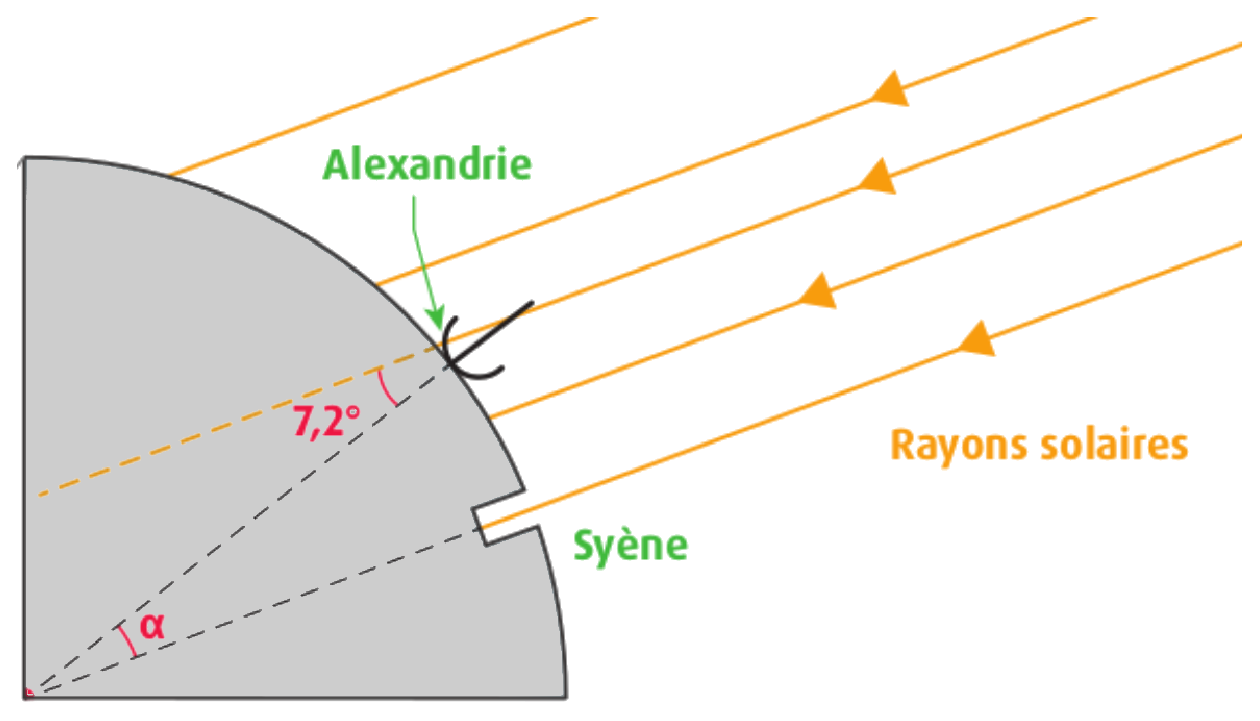
\includegraphics[width=8.5cm]{methode_eratosthene}
      & &
      Diamètre de la Terre à l'équateur : 12 756 km \newline
      Circonférence de la Terre : 40 075 km \newline
      Surface de la Terre : 510 065 700 km$^2$ \newline
      Âge de la Terre : 4,566 milliards d'années \newline
      Altitude maximale : 8 850 m \newline
      Profondeur maximale : $-$ 11 035 m \newline
      \begin{center}
         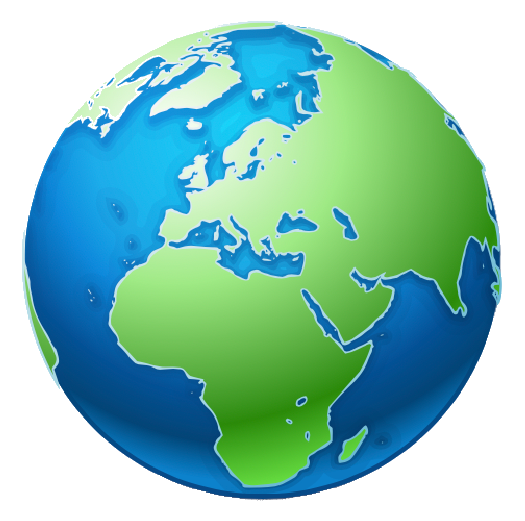
\includegraphics[width=5cm]{Terre}
      \end{center}
     \\
      \cline{1-1} \cline{3-3}
   \end{tabular}}
}